\chapter{Evaluation} \label{evaluation}

In diesem Kapitel werden \PSCORM, Kohana und Doctrine in einem Benchmark verglichen. Dabei wird der automatisch generierte Code der zweiten Ebene von \PSCORM genutzt. Teile dieser Demo-Applikation sind im Anhang \ref{tests-code} zu finden. Kohana und Doctrine wurden so konfiguriert, wie in ihren Dokumentationen angegeben. Im ersten Kapitel stelle ich die Konfiguration des Testsystems vor. Danach werden beide Tests mit einigen Implementierungsdetails vorgestellt. Im letzten Kapitel befindet sich die Auswertung des Benchmarks.

\section{Konfiguration}
Das Beispiel aus dem Kapitel \ref{object-loading} wurde als erster Test genommen. Es werden alle Tests in allen Applikationen (Kohana, Doctrine, \PSCORM) durchgeführt und ihre Laufzeit gemessen. Dabei wird die Laufzeit als arithmetisches Mittel über mindestens 5 voneinander unabhängige Aufrufe des Tests errechnet\footnote{dies geschieht um Schwankungen auf dem Hostsystem auszugleichen}. Die Ergebnisse der Tests sind in [\ref{evaluation-results}] zu sehen. Die Tests wurden auf einem Hostsystem mit folgender Konfiguration ausgeführt:
\begin{itemize}
\item AMD Athlon 64 X2 Dual Core Prozessor 4800+ (2 x 2,41 GHz)
\item 2GB RAM
\item Microsoft Windows XP Professional 32 Bit Service Pack 3
\item PHP 5.3.3 (VC6 Thread Safe)
\item MySQL 5.0.41-community-nt
\item APC 3.1.5-dev 
\item Xdebug v2.1.0
\end{itemize}
Alle nicht notwendigen Prozesse wurden während der Tests ausgeschaltet. Die Laufzeiten wurden mit dem XDebug-Profiler aufgezeichnet und mit Wincachegrind\footnote{Version 1.0.0.12} ausgewertet. Da der Schwerpunkt der Analyse auf die Performanz der PHP Applikation gelegt werden soll, wurde der Anfragencache von MySQL deaktiviert. Der Opcode-Cache \term{APC} wurde für alle Skripte aktiviert und so benutzt, dass die erste Auswertung bereits mit einem warmen Opcode-Cache startete.

\section{Test 1}
In Test 1 und Test 2 sollen alle \object{Aggregation2Project}-Objekte inklusive der Unterobjekte \object{Project} und \object{Aggregation} instanziiert werden. In Test 1 werden die drei Objekte jeweils einzeln konstruiert:\\
\begin{enumerate}
\item Lade alle Objekte der Relation \tabelle{projects}. \\
\item Lade alle Objekte der Relation \tabelle{aggregations}. \\
\item Lade alle Objekte der Relation \tabelle{aggregations\_projects}. Lade zusätzlich die Informationen für die Unterobjekte \object{Project} und \object{Aggregation}.
\item Zeige die Informationen aller \object{Aggregation2Project}-Objekte mit deren Unterobjekten an.
\end{enumerate}
Damit das Anzeigen der Daten im letzten Schritt in jedem Test und jedem Aufruf gleich ist, wird ein Anzeigeskript am Ende jedes Tests aufgerufen (Quelltext \ref{print_objects}). Die Applikation selbst muss einen Array (\code{\$objects}) von allen \object{Aggregation2Project}-Objekten zurückgeben. \\
\begin{fcode}[bhtp]
    \lstset{style=php}
    \begin{lstlisting}
    foreach ($objects as $test) {
      print $test->getProject()->getName();
      print '('.$test->getProject()->getListvisible().')  ';
      print $test->getSeconds().' '.$test->getShare().'   ';
      print $test->getAggregation()->getClosed();
      print '<br />';
    }
    \end{lstlisting}
    \caption{print\_objects.php: Die Daten jedes Tests werden ausgegeben}
\label{print_objects}
\end{fcode}%$
Wenn die Applikation von einem Cache Gebrauch macht, ist die Objektidentität gewährleistet und die Unterobjekte des Objektes \object{Aggregation2Project} werden aus dem Cache geladen, so dass bei der Ausgabe keine weiteren Anfragen an die Datenbank nötig sind. Im Anhang \ref{tests-code} ist der entscheidene Teil des Quelltextes der Applikationen abgebildet. Ich fasse die Vorgehensweisen der einzelnen Applikationen für die jeweiligen Tests kurz zusammen, so dass die Quelltexte nur für Interessierte wichtig sind: 
\paragraph{Kohana}
In Kohana ist es nicht möglich einen Cache zu benutzen. Der Entwickler müsste selbst dafür sorgen, dass die Objekte die in 1. und 2. geladen werden, nicht erneut beim Instanziieren von \object{Aggregation2Project}-Objekten nachgeladen werden. Dieses Problem wurde in diesem Test nicht berücksichtigt, da ein Entwickler ohne die Kentnisse über die Interna von Kohana diesen Fehler ebenfalls begehen würde. Schritt 1 und Schritt 2 wurden dann weggelassen, da beide Schritte auf die Ausführung von Schritt 3 keinen Einfluss haben. In Kohana wird also nur Schritt 3 ausgeführt und im Anzeigeskript werden dann die \object{Project}-Objekte und \object{Aggregation}-Objekte dynamisch nachgeladen (\term{Lazy-Loading}.
\paragraph{\PSCORM}
Aus der \term{Query}-Klasse wird \code{getAllAggregation2Project()} aufgerufen. Es werden zuerst alle Objekte aus \tabelle{projects} dann aus \tabelle{aggregations} hydratet. Der Cache von \PSCORM nimmt alle Objekte auf, die in diesen Funktionen mit \code{populate()} übergeben werden. Danach werden die Unterobjekte beim Instanziieren von den \object{Aggregation2Project}-Objekten jeweils aus dem Cache referenziert. 
\paragraph{Doctrine}
In Doctrine ist der Ablauf ähnlich wie in \PSCORM. Durch sogenannte \term{Entity-Repositories} können Objekte von einer gesamten Tabelle geladen werden. Es werden zuerst alle Objekte aus \tabelle{projects} geladen dann von \tabelle{aggregations}, ohne das Ergebnis dieser Abfragen zu untersuchen. Danach werden alle Einträge aus \tabelle{aggregations\_projects} in Objekte umgewandelt. Da man die SQL Befehle die Doctrine absetzt, ausgeben kann, sieht man, dass nach einmaligen Laden von z.~B. \tabelle{projects} keine weiteren Abfragen auf diese Tabelle gemacht werden. Da die Unterobjekte in dem Ergebnis der dritten Abfrage von \tabelle{aggregations\_projects} aber korrekt instanziiert sind, muss Doctrine diese Objekte aus einem eigenen Cache geladen haben\footnote{So wird es auch in der Dokumentation erklärt}. \\

\section{Test 2}

Der zweite Test unterscheidet sich dadurch, dass nun nicht mehr die Unterobjekte von \tabelle{projects} und \tabelle{aggregations} vorher geladen werden sollen. Der Applikation soll es erlaubt sein in einem großen Query alle Informationen auf einmal abzufragen. Die Ausgabe soll aber dieselbe sein wie für Test 1.
\begin{enumerate}
\item Lade alle Objekte der Relation \tabelle{aggregations\_projects}. Lade zusätzlich die Informationen für die Unterobjekte \object{Project} und \object{Aggregation}
\item Zeige die Informationen aller \object{Aggregation2Project}-Objekte mit deren Unterobjekten an
\end{enumerate}
\paragraph{Kohana}
In Kohana ist es möglich das \term{Lazy Loading} wie in Test 1 manuell zu unterbinden. Beim Erstellen der Abfrage für die \object{Aggregation2Project}-Objekte kann man angeben, welche Unterobjekte durch einen Join mitgeladen werden sollen. Dies geschieht durch die Funktion \code{with()}\footnote{In Beispiel \ref{kohana-sql-api} in Kapitel \ref{frameworks} ist dies zu sehen}. Das die Objekte nicht mehr mit eigenen Abfragen nachgeladen werden, kann man am SQL-Log der Applikation sehen.
\paragraph{\PSCORM}
Zu Demonstrationszwecken für den Test 2 wurde eine ähnliche Funktionalität wie bei Doctrine und Kohana hinzugefügt. Die Klasse QueryTest2 führt in \code{getAllAggregation2Project()} einen Join über alle drei Tabellen aus und gibt dann jeweils den gesamten Datensatz an alle Unterobjekte weiter, um \code{init()} aus\-füh\-ren zu können. Bevor \code{init()} von \object{Aggregation2Project} aufgerufen wird, sind die Unterobjekte dem Cache bereits bekannt gemacht wurden, so dass die \code{init()}-Funktion von \object{Aggregation2Project} auf die Objekte im Cache zurückgreifen kann. Wie in Kapitel \ref{object-loading} gezeigt, ist dies aber die langsamere Methode in \PSCORM Objekte zu laden. Diese Funktionalität wurde deshalb wurde nur zum Vergleich zu den anderen Frameworks hier aufgenommen.
\paragraph{Doctrine}
In Doctrine wird die Anfrage in DQL geschrieben. Dabei kann man mit 2 \term{fetch Joins} bestimmen, dass die Daten für die Unterobjekte für \object{Aggregation2Project} direkt mitgeladen werden. Im SQL-Log sieht man, dass nur eine Abfrage mit 2 \term{JOINS} ausgeführt wird und keine weiteren Abfragen abgesetzt werden.

\section{Ergebnisse} \label{evaluation-results}

Auf der Y-Achse des Diagrammes in Abbildung \ref{evaluation-results-bild} ist die Laufzeit der verschiedenen Tests in Millisekunden aufgetragen. Kohana braucht für Test 1 ungefähr 11 Sekunden. Doctrine und \PSCORM lösen Test 1 im Sekundenbereich (1,4s und 0,7s). \\
Test 2 verbraucht bei Doctrine und \PSCORM mehr Ressourcen und Zeit als Test 1. Kohana verbessert sich und benötigt ungefähr 6,5s, Doctrine 1,8s und PSCORM 1,1s. \\
\begin{figure}[h!]
  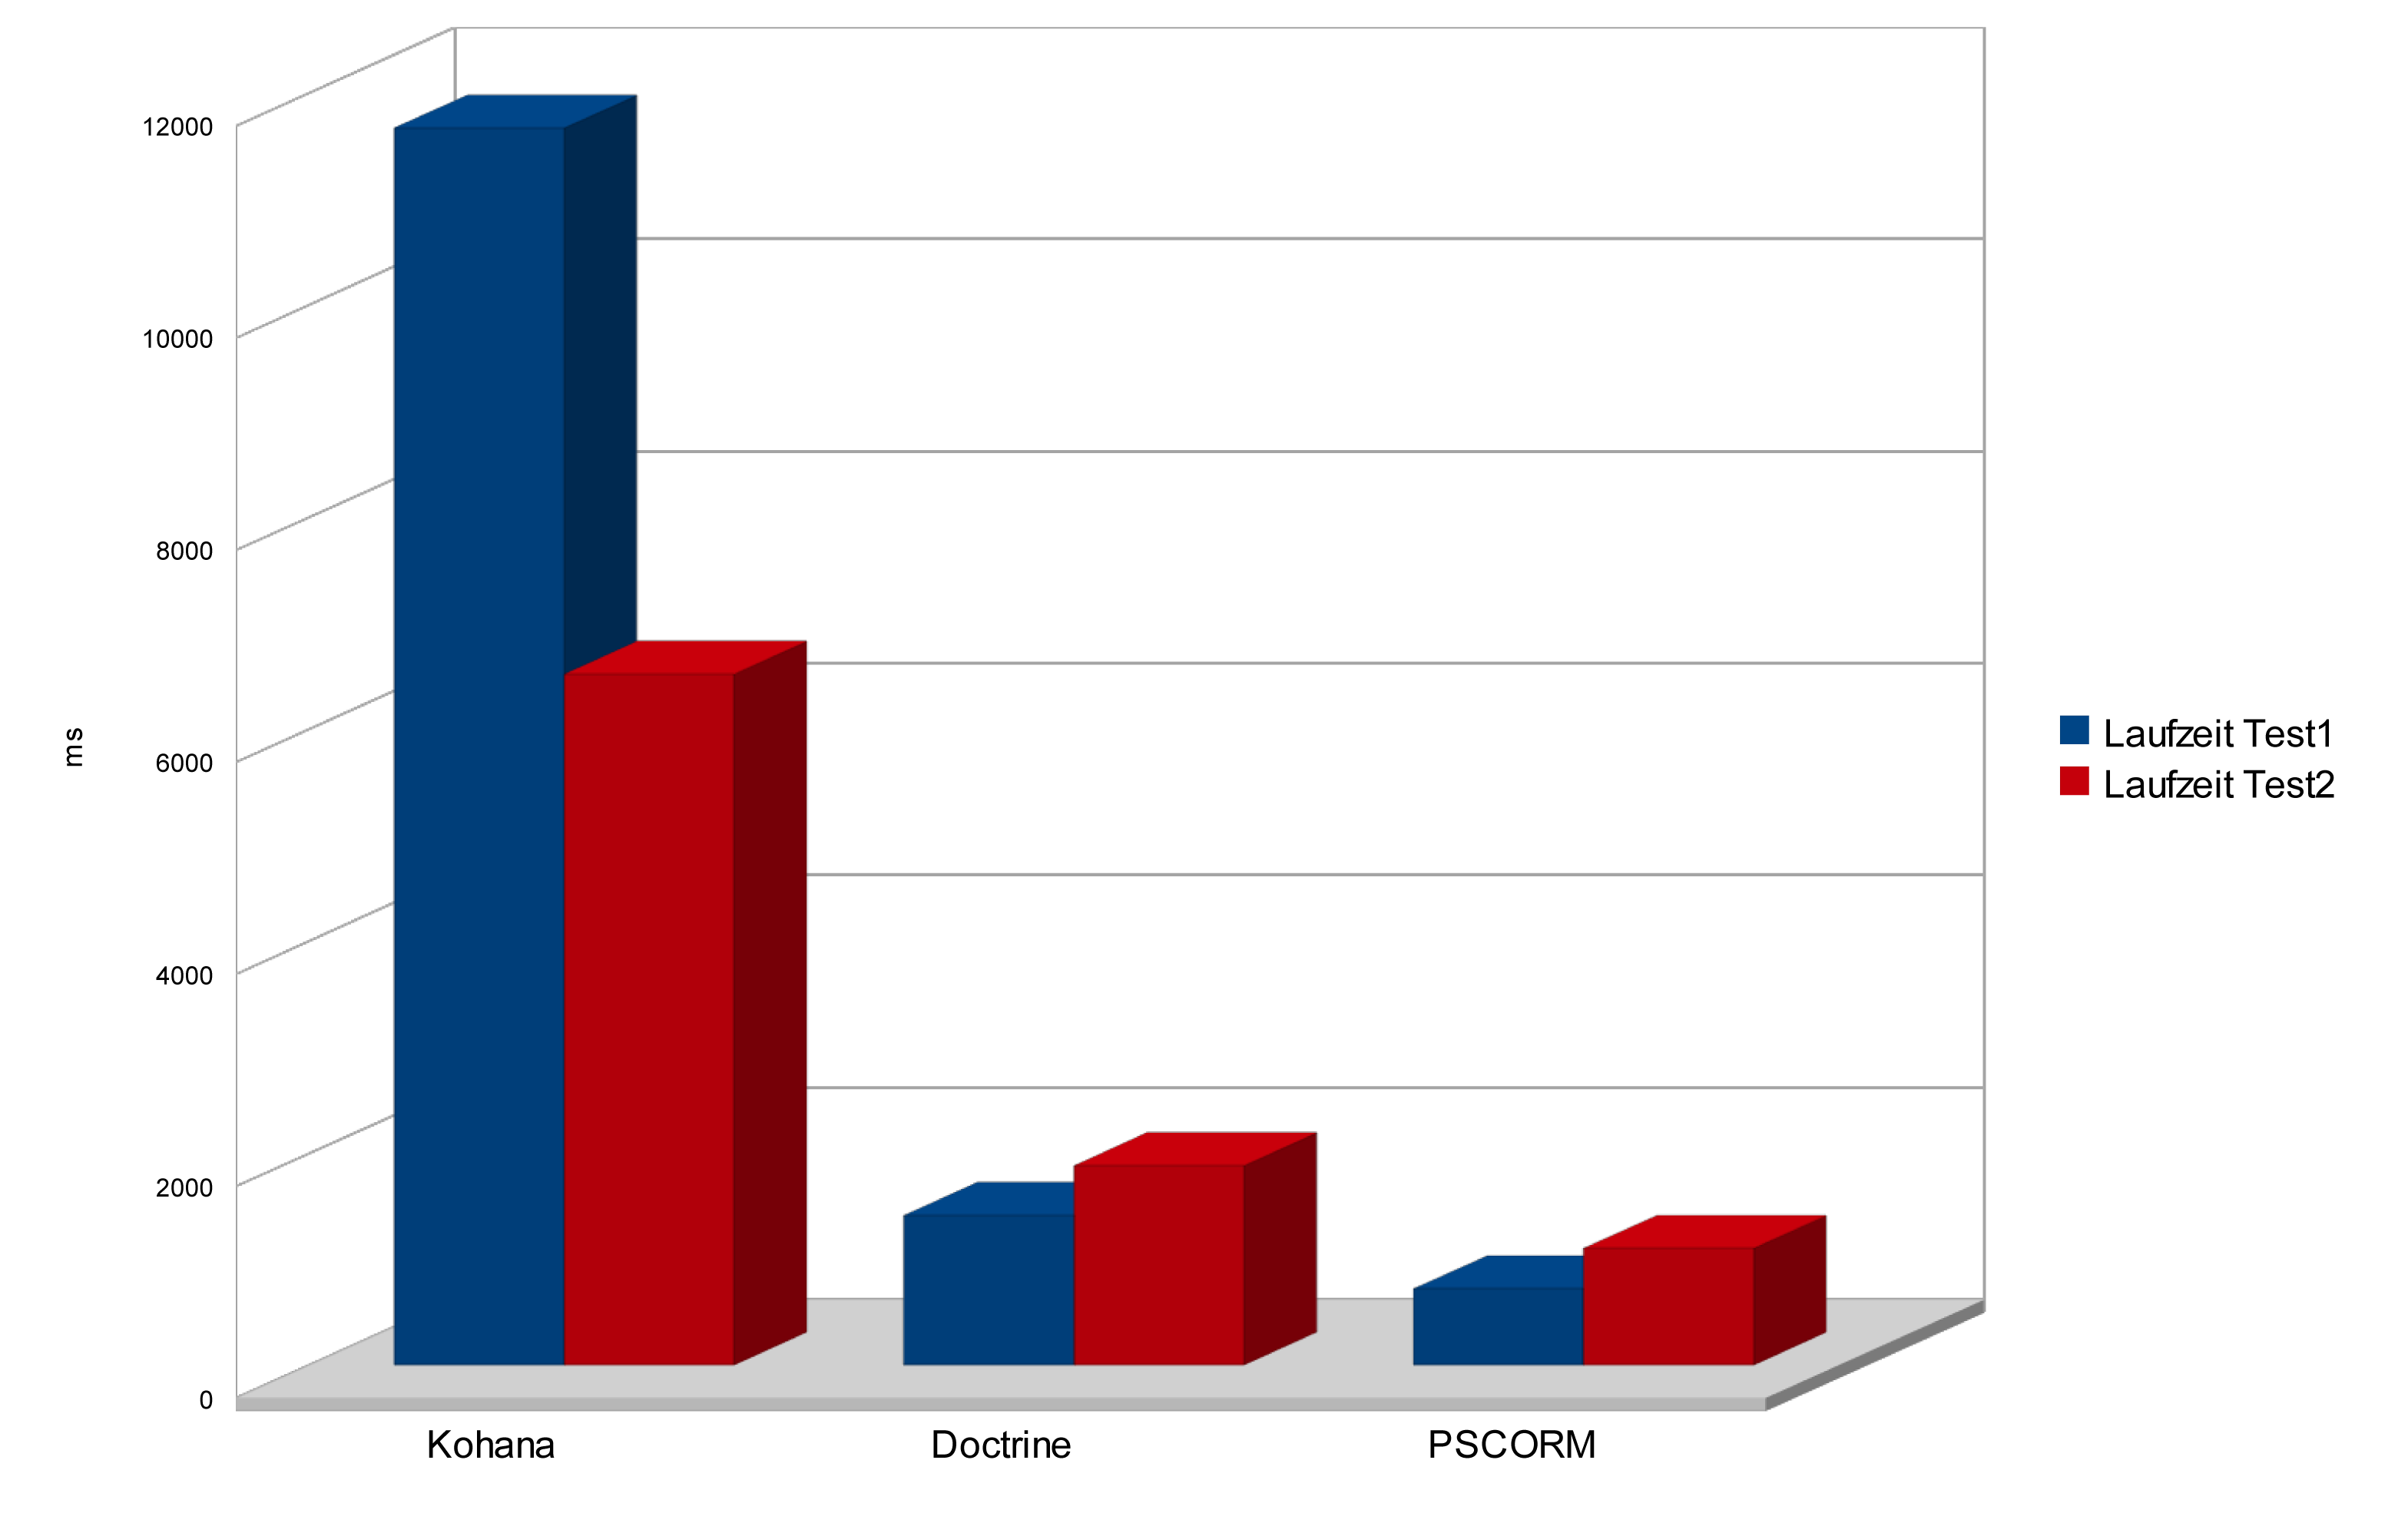
\includegraphics[width=\textwidth]{figures/evaluation}
  \caption{Auswertung der Laufzeiten für die Tests}
  \label{evaluation-results-bild}
\end{figure}
\noindent Zuerst fällt also auf, dass Kohana fast das zehnfache an Zeit für den ersten Test braucht und sich beim zweiten Test verbessern kann, während \PSCORM und Doctrine sich leicht verschlechtern. Wie schon beschrieben, ist es nicht möglich einen Cache für die Objekte in Kohana\footnote{zumindest nicht in Version 2.4} zu benutzen. Es gibt zwar die Möglichkeit einen APC-Cache anzusprechen, man müsste aber die komplette Logik für die Objekte selbst schreiben. Außerdem ist es nicht möglich in den Prozess des \term{Object-Marshalling} einzugreifen, so dass die Funktionen von Kohana gar nicht von einem \objectcache profitieren könnten.\\
Zur Erinnerung: in \tabelle{aggregations\_projects} gibt es 11.862 Tupel. Diese müssen in beiden Tests als Objekte geladen werden. Jedes Objekt besitzt zwei weitere Unterobjekte. Da Kohana keinen Cache benutzen kann, muss das Framework 11.862 * 2 Einzelanfragen der Form \code{SELECT * FROM aggregation|project WHERE id = :id} an die Datenbank stellen und daraus 11.862 * 3 Objekte herstellen. Die schlechte Laufzeit ist die Konsequenz von dem, was im Kapitel \ref{object-loading} über das Object-Loading festgestellt wurde: Zu viele \term{Roundtrips} an die Datenbank verschlechtern die Performanz erheblich. \PSCORM und Doctrine führen nur 1 + [Kardinalität von \tabelle{projects})] + [Kardinalität von \tabelle{aggregations}] Anfragen an die Datenbank aus. Davon hydrieren sie nur so viele Objekte wie es Tupel in der Datenbank gibt: 11.862 + 193 (\object{Projects}) + 3.742 (\object{Aggregations}) = 15797 Objekte. Kohana hydriert dagegen die mehr als doppelte Anzahl von 35.586 Objekten. \\
Dies erklärt auch direkt, warum Kohana im zweiten Test besser wird. Da es die Daten direkt in der Abfrage für die \object{Aggregation2Project}-Objekte mit einem Join mitlädt, entfallen die mehr als 22.000 simplen Einzelabfragen an die Datenbank. Trotzdem muss es noch die gleiche Anzahl an Objekten aus diesem Query erstellen. \\
\\
Warum ist \PSCORM noch ein bisschen schneller als Doctrine in beiden Tests? Wie im einleitenden Kapitel \ref{besonderheiten-php} über PHP-Webapplikationen beschrieben, gewinnt man Performanz, wenn man den Code möglichst einfach hält und besonders wenig mit Klassen oder Funktionen abstrahiert. Die Klassen von \PSCORM auf denen die Tests ausgeführt wurden, sind eigentlich automatisch generierte (kompilierte) Codeteile\footnote{Für diese Tests wurden sie dennoch von Hand geschrieben}. Während Doctrine die DQL-Anfrage noch in SQL umwandeln muss, benutzt \PSCORM eine als String hartcodierte Anfrage, die vorher durch den Export des Projektes erstellt wurde. Diese muss zur Laufzeit nicht erst dynamisch von PHP-Funktionen oder Klassen zusammengebaut werden. Doctrine opimiert dieses Parsen der DQL-Anfrage, indem es den APC Cache benutzt. Der Vorteil durch das Benutzen von möglichst simplen Code von \PSCORM zeigt sich aber auch beim Hydrieren von Objekten: Doctrine muss hier Klassen instanziieren, um die speziellen und die Basismappings für die Umwandlung von einem Wert einer Spalte der Datenbankrelation in einen Wert der objektorientierten Applikation vornehmen zu können. In \PSCORM wird der Code direkt verwendet, weil er dynamisch in die \code{init()}-Funktion eingebunden wurde. \PSCORM führt also zur Umwandlung eines Strings aus der Datenbank in einen Integer in PHP nur einen Typcast aus, während Doctrine die (gecachten) Metadaten für die Spalte auslesen muss, die Klasse für das Mapping instanziieren muss und die Funktion zur Umwandlung aufruft. Auch wenn der Performanzunterschied mit Caching und Wiederverwendung des Mappings zwar stark reduziert werden kann, muss man bedenken, dass dieses Mapping im Test 1, wenn es im \object{Aggregation2Project}-Objekt benutzt wird, 11.000 mal ausgeführt wird. Ein Gewinn von wenigen Millisekunden kann dann schon große Auswirkungen haben.\\
\\
Es ist zu beachten, dass diese Evaluation nur ein Test für einen Teil der Leistungsfähigkeit der Frameworks ist. Die gesamte Skalierbarkeit dieser Applikationen müsste durch viel umfangreichere Benchmarks überprüft werden. Die vorgestellten Ergebnisse konzentrieren sich hauptsächlich auf das Laden von Objekten. Hierbei wird nur ein Fall von vielen Beleuchtet. Andere denkbare Tests wären das Laden mit Collections, das Laden von größeren verschachtelten Strukturen oder die Bearbeitung von Aggregationsfunktionen\footnote{solche Funktionen wie SUM() oder AVG(), die bereits auf der Datenbankebene mehrere Datensätze von Objekten zu einem neuen Ergebnis aggregieren}. Weitere Tests aus anderen Bereichen könnten z.~B. die Leistungsfähigkeit der Vererbung oder des Caches sein. Man kann sich weitere Szenarios vorstellen. Deshalb ist nicht auszuschließen, dass die Performanz der anderen Frameworks gegen über \PSCORM für andere Testfälle besser ist.\\
